\documentclass[11pt]{article}

\usepackage[letterpaper,margin=1in]{geometry}
\usepackage{amsmath,amssymb}
\usepackage{graphicx}
\usepackage{booktabs}
\usepackage{microtype}
\usepackage{xcolor}
\usepackage[colorlinks=true,linkcolor=navyblue,urlcolor=navyblue,citecolor=navyblue]{hyperref}
\usepackage{titlesec}
\usepackage{caption}
\usepackage[T1]{fontenc}
\usepackage{lmodern}

\definecolor{navyblue}{HTML}{1A3A5C}

\titleformat{\section}{\Large\bfseries\color{navyblue}}{\thesection.}{0.5em}{}
\titleformat{\subsection}{\large\bfseries\color{navyblue}}{\thesubsection.}{0.5em}{}
\titlespacing*{\section}{0pt}{1.5em}{0.5em}
\titlespacing*{\subsection}{0pt}{1em}{0.3em}

\captionsetup{font=small,labelfont=bf,format=hang}

\setlength{\parskip}{0.5em}
\setlength{\parindent}{0pt}

\graphicspath{{../output/figures/}}

\title{\bfseries Juvenile Red King Crab $\times$ Ocean Acidification: an interim meta-analysis}
\author{Mike Litzow \\ \textit{NOAA Alaska Fisheries Science Center}}
\date{\today}

\begin{document}

\maketitle

\begin{abstract}
\noindent Three laboratory experiments at the Kodiak Laboratory have exposed juvenile red king crab (\textit{Paralithodes camtschaticus}) to combinations of reduced pH and elevated temperature. Two are published (Long et al.\ 2013; Swiney et al.\ 2017) and one (2024--25) is unpublished. This document reports the first joint Bayesian analysis of survival and wet-mass growth across all three studies, develops a Weibull-hazard survival model that decisively outperforms the constant-hazard model used by the source papers, tests whether initial wet mass or threshold pH effects mediate the experiment-level differences, and contrasts a published-only analysis (Model A) with an all-three-experiment analysis (Model B) at every stage.
\end{abstract}

% ============================================================
\section{Goals}
% ============================================================

Five specific goals:
\begin{enumerate}
\item[(i)] Bring the raw survival and growth records into a common, audit-ready structure that can be extended with future experiments.
\item[(ii)] Quantify the effects of mean pH and mean temperature on daily mortality, contrasting Model A (published only) with Model B (all three).
\item[(iii)] Evaluate whether tank-level differences in initial wet mass mediate the experiment-level mortality differences identified in Model B.
\item[(iv)] Make the same A-vs-B contrast for wet-mass growth using pH and temperature as covariates, and ask whether initial mass mediates the experiment-level growth differences.
\item[(v)] Test for nonlinear / threshold effects of pH on both survival and growth using Bayesian thin-plate smooths.
\end{enumerate}

% ============================================================
\section{Methods}
% ============================================================

\subsection{Data sources and preparation}
Raw data from the three experiments were obtained as Excel workbooks from the Kodiak Laboratory archive. All sheets were converted to CSV. A single script (\texttt{scripts/data\_wrangling.R}) ingests the CSVs and produces three harmonised tables: a daily-survival panel, an individual-level wet-mass panel, and a treatment-conditions table with the realised mean pH and mean temperature for each tank. Realised conditions were computed from daily pH and temperature records for 2012 and 2024; for 2010 the means and SDs reported in Long et al.\ 2013 (Table~1) are used because no daily file is in the archive. Table~\ref{tab:cond} lists the realised conditions for all seventeen tanks.

\begin{table}[h]
\centering\small
\begin{tabular}{lllrr}
\toprule
Experiment & pH treat. & Temp treat. & Mean pH (SD) & Mean temp $^\circ$C (SD) \\
\midrule
2010-2011 & ambient & ambient & 8.040 (0.040) & 9.1 (2.0) \\
2010-2011 & pH 7.8  & ambient & 7.802 (0.025) & 9.1 (2.0) \\
2010-2011 & pH 7.5  & ambient & 7.503 (0.040) & 9.1 (2.0) \\
2012-2013 & ambient & ambient & 7.99 (0.03)   & 8.38 (1.62) \\
2012-2013 & ambient & +2C     & 7.96 (0.04)   & 10.2 (1.49) \\
2012-2013 & ambient & +4C     & 7.94 (0.04)   & 12.2 (1.63) \\
2012-2013 & pH 7.8  & ambient & 7.79 (0.02)   & 8.55 (1.49) \\
2012-2013 & pH 7.8  & +2C     & 7.76 (0.02)   & 10.4 (1.49) \\
2012-2013 & pH 7.8  & +4C     & 7.74 (0.01)   & 12.3 (1.62) \\
2024-2025 & ambient & ambient & 7.88 (0.03)   & 8.53 (2.08) \\
2024-2025 & ambient & +3C     & 7.88 (0.06)   & 10.3 (2.06) \\
2024-2025 & pH 7.55 & ambient & 7.56 (0.03)   & 7.43 (1.92) \\
2024-2025 & pH 7.55 & +3C     & 7.54 (0.03)   & 10.4 (2.09) \\
2024-2025 & pH 7.65 & ambient & 7.67 (0.03)   & 7.42 (1.92) \\
2024-2025 & pH 7.65 & +3C     & 7.65 (0.03)   & 10.2 (2.06) \\
2024-2025 & pH 7.85 & ambient & 7.88 (0.05)   & 7.41 (1.91) \\
2024-2025 & pH 7.85 & +3C     & 7.85 (0.10)   & 10.3 (2.25) \\
\bottomrule
\end{tabular}
\caption{Realised treatment conditions.}
\label{tab:cond}
\end{table}

\subsection{Data-entry corrections}
Audit of the 2024--25 worksheet uncovered thirteen data-entry anomalies. Proposed corrections were documented in \texttt{documents/2024-2025\_data\_issues\_for\_review.docx} and reviewed by the original data holder (C.\ Long, NOAA AFSC) via track changes. Confirmed corrections are applied as documented \texttt{fix\_cell\_24()} calls in the wrangling script, keyed by (tub, cell). Two are non-trivial. The ambient/ambient tub in 2024 (Tub~7) experienced a flow-cut event on 2024-12-16 that killed 14 of 15 crabs simultaneously, so that series is censored at the day before the failure (day~117). Two crabs flagged as ``missing, not dead, remove from analysis'' are dropped from both survival and growth analyses, reducing the starting count for their tanks by one. Two 2012 wet-mass measurements at \texttt{exp\_day}~=~505 and~508 (the experiment ran 184 days) are clearly date-entry errors and are dropped from the growth analysis.

\subsection{Validation against published results}
Before extending the analysis, the cleaned data were checked against the values reported in the two source papers. A constant-hazard maximum-likelihood fit to the cleaned data reproduces the per-treatment mortality rates of Long et al.\ 2013 to within rounding (within 1\% on every rate). An exponential growth model on log wet mass with a per-crab random intercept reproduces the published $a$ and $b$ coefficients (within 4\% on the slope). The relative effects of pH and temperature on 2012--13 mortality reported by Swiney et al.\ 2017 and their survival ranking across treatments both reproduce exactly. The reproduction code lives at \texttt{scripts/check\_against\_papers.R}.

\subsection{Survival model}
\label{sec:surv_model}
Daily counts of live crabs were modelled with a Bayesian binomial hazard formulation. Two parameterisations were considered. A \emph{constant-hazard} model assumes that per-tank rate $r_i$ does not vary with time:
\begin{equation}
P(\text{alive at } t \mid \text{tank } i) = \exp(-r_i \, t).
\end{equation}
A \emph{Weibull} model lets the hazard rise (or fall) with time-since-start through a shape parameter $k$:
\begin{equation}
P(\text{alive at } t \mid \text{tank } i) = \exp\!\left(-(r_i \, t)^k\right).
\end{equation}
Weibull reduces to constant hazard when $k = 1$. Both admit the same daily-binomial likelihood. Using the complementary log-log link, the linear predictor is $k \log(t)$ plus the covariate sum, so constant hazard is implemented with \texttt{offset(log(t))} and Weibull lets $\log(t)$ enter as a free coefficient whose value estimates $k$:
\begin{align}
n^{\text{died}}_{i,t} \mid n^{\text{init}}_i &\sim \text{Binomial}\!\left(n^{\text{init}}_i, \mu_{i,t}\right), \\
\operatorname{cloglog}(\mu_{i,t}) &= k\log t + \beta_0 + \beta_{\text{exp}} \cdot \text{exp}_i + \beta_{\text{pH}}\,\text{pH}^c_i + \beta_T\,\text{temp}^c_i \nonumber\\
&\quad + \beta_{\text{int}}\,\text{pH}^c_i \cdot \text{temp}^c_i + u_i,\\
u_i &\sim \text{Normal}(0, \sigma_{\text{tank}}).
\end{align}
Centering values were $\text{pH}^c = \text{pH} - 8.0$ and $\text{temp}^c = \text{temp} - 10^\circ$C. \textit{exp} is a categorical for experiment (2010--11 reference). $u_i$ is a tank-level random intercept; with one tank per treatment it is the closest available analogue to a treatment-level replicate.

Priors were weakly informative: $\beta_0 \sim \text{Normal}(-5, 2)$; all other slopes $\sim \text{Normal}(0, 5)$; $k \sim \text{Normal}(1, 0.5)$; $\sigma_{\text{tank}} \sim \text{Exponential}(1)$. Models were fit in R 4.6 with \texttt{brms} 2.23 calling Stan via \texttt{rstan}: four chains of 3{,}000 iterations (1{,}500 warmup); \texttt{adapt\_delta} = 0.95 (0.97 for Weibull); manual init anchoring the intercept near $-5$. Model comparison uses leave-one-out cross-validation (LOO) via the \texttt{loo} package.

\subsection{Initial-mass covariate (survival)}
The Weibull survival model was extended with the centred log tank-mean initial wet mass as a fixed-effect covariate, to test whether tank-level differences in initial size mediate the experiment-level mortality differences. Per-tank means are computed from molt~0 records; the missing 2010 pH~7.5 mean is imputed as the average of the other two 2010 tanks (all 2010 crabs came from a single Bristol Bay cohort).

\subsection{Growth model}
\label{sec:growth_model}
Wet-mass measurements were modelled with a Bayesian log-linear growth model. Following Long et al.\ 2013 the working assumption is exponential growth: $\log(\text{WM})$ linear in time, with per-crab random intercepts to absorb individual size variation. \textbf{The time variable is experimental days, not degree days}, so that temperature can be identified as a free covariate rather than absorbed by the time axis. The growth rate (slope on \texttt{exp\_day}) is allowed to vary with experiment, pH, and temperature through interactions:
\begin{align}
\log(\text{WM}_{c,t}) &= (\beta_0 + \beta_{\text{exp}} \text{exp} + \beta_{\text{pH}} \text{pH}^c + \beta_T \text{temp}^c + \beta_{\text{int}}\text{pH}^c \text{temp}^c) \nonumber\\
&\quad + (\delta_0 + \delta_{\text{exp}} \text{exp} + \delta_{\text{pH}} \text{pH}^c + \delta_T \text{temp}^c + \delta_{\text{int}}\text{pH}^c \text{temp}^c) \cdot \text{day}_{c,t} \nonumber\\
&\quad + a_{\text{crab}} + u_{\text{tank}} + \epsilon_{c,t}, \\
a_{\text{crab}} &\sim \text{Normal}(0, \sigma_{\text{crab}}), \\
u_{\text{tank}} &\sim \text{Normal}(0, \sigma_{\text{tank}}), \\
\epsilon_{c,t} &\sim \text{Normal}(0, \sigma).
\end{align}
The $\beta$ terms set the intercept (log initial mass) per experiment/treatment; the $\delta$ terms set the growth rate per day per experiment/treatment. The per-crab random intercept $a_{\text{crab}}$ is the analog of Long et al.'s ``$a$ varies with crab number''. Priors: $\beta_0 \sim \text{Normal}(-5, 1)$ (roughly $\log 0.01$~g); all other slopes $\sim \text{Normal}(0, 1)$; random-effect SDs $\sim \text{Exponential}(2)$.

\subsection{Smooth pH (threshold) extension}
\label{sec:smooth_model}
To test for nonlinear / threshold effects of pH, both survival and growth models were refit with the linear pH terms (and pH$\times$temp interaction) replaced by a Bayesian thin-plate spline (\texttt{s(mean\_pH, k = 5)}). Temperature was held as a linear covariate, per the design intent of letting pH vary while holding temperature effects constant. For growth, the smooth was added both as an intercept term (\texttt{s(mean\_pH)}) and as a growth-rate term (\texttt{s(mean\_pH, by = exp\_day)}); the latter encodes that growth rate per day varies smoothly with pH. A Student-$t(3, 0, 1)$ prior is placed on the smooth-wiggliness SD. Comparison to the linear-pH fits uses LOO.

% ============================================================
\clearpage
\section{Results}
% ============================================================

\subsection{Weibull vs constant-hazard model comparison}
All four base survival fits (constant and Weibull, Models A and B) converged cleanly (max $\hat R \le 1.01$; minimum bulk ESS $\ge 1{,}355$). LOO decisively prefers Weibull in both designs (Table~\ref{tab:loo-weibull}): $\Delta$ELPD $= -1{,}404$ (Model A) and $-1{,}726$ (Model B), both at SE $\approx 70$.

\begin{table}[h]
\centering\small
\begin{tabular}{llrr}
\toprule
Design & Hazard model & $\Delta$ ELPD & SE \\
\midrule
Model A (published only) & Weibull & 0 & 0 \\
                          & Constant hazard & $-1{,}404$ & 69 \\
\midrule
Model B (all 3 experiments) & Weibull & 0 & 0 \\
                            & Constant hazard & $-1{,}726$ & 75 \\
\bottomrule
\end{tabular}
\caption{LOO ELPD differences. Weibull preferred by $>20$~SE in both designs.}
\label{tab:loo-weibull}
\end{table}

The Weibull shape parameter is $k = 1.98$ [1.94, 2.02] in both designs, sharply excluding $k = 1$. With $k \approx 2$ the cumulative hazard scales as $t^2$: the instantaneous mortality rate rises roughly linearly with time. A crab that has survived 100 days has on the order of four times the daily mortality risk it had at day 25. All remaining survival analyses use the Weibull formulation. The constant-hazard fit is retained only for paper-validation.

\subsection{Survival Model A: published experiments only}
\label{sec:results-a}
Fixed-effect posteriors are shown in Table~\ref{tab:surv-A}. The pH main effect is strongly negative and its credible interval narrowly excludes zero; the temperature main effect and pH$\times$T interaction are uninformative. There is no detectable baseline difference between 2010 and 2012.

\begin{table}[h]
\centering\small
\begin{tabular}{lrr}
\toprule
Parameter & Median & 95\% CI \\
\midrule
Weibull shape $k$ (log\_day coef.) & 1.98 & 1.94, 2.02 \\
Intercept (log $r$ at pH 8.0, 10$^\circ$C, 2010) & $-10.37$ & $-11.65, -9.08$ \\
Experiment 2012 vs 2010 & 0.01 & $-1.40, 1.37$ \\
pH (per unit; centred at 8.0) & $-3.98$ & $-7.46, -0.07$ \\
Temperature (per $^\circ$C; centred at 10$^\circ$C) & 0.20 & $-0.45, 0.88$ \\
pH $\times$ Temperature interaction & 0.80 & $-2.69, 4.18$ \\
Tank-level SD & 0.77 & 0.39, 1.61 \\
\bottomrule
\end{tabular}
\caption{Survival Model A (Weibull) fixed-effect posteriors. Values on the log mortality-rate scale.}
\label{tab:surv-A}
\end{table}

\begin{figure}[h]
\centering
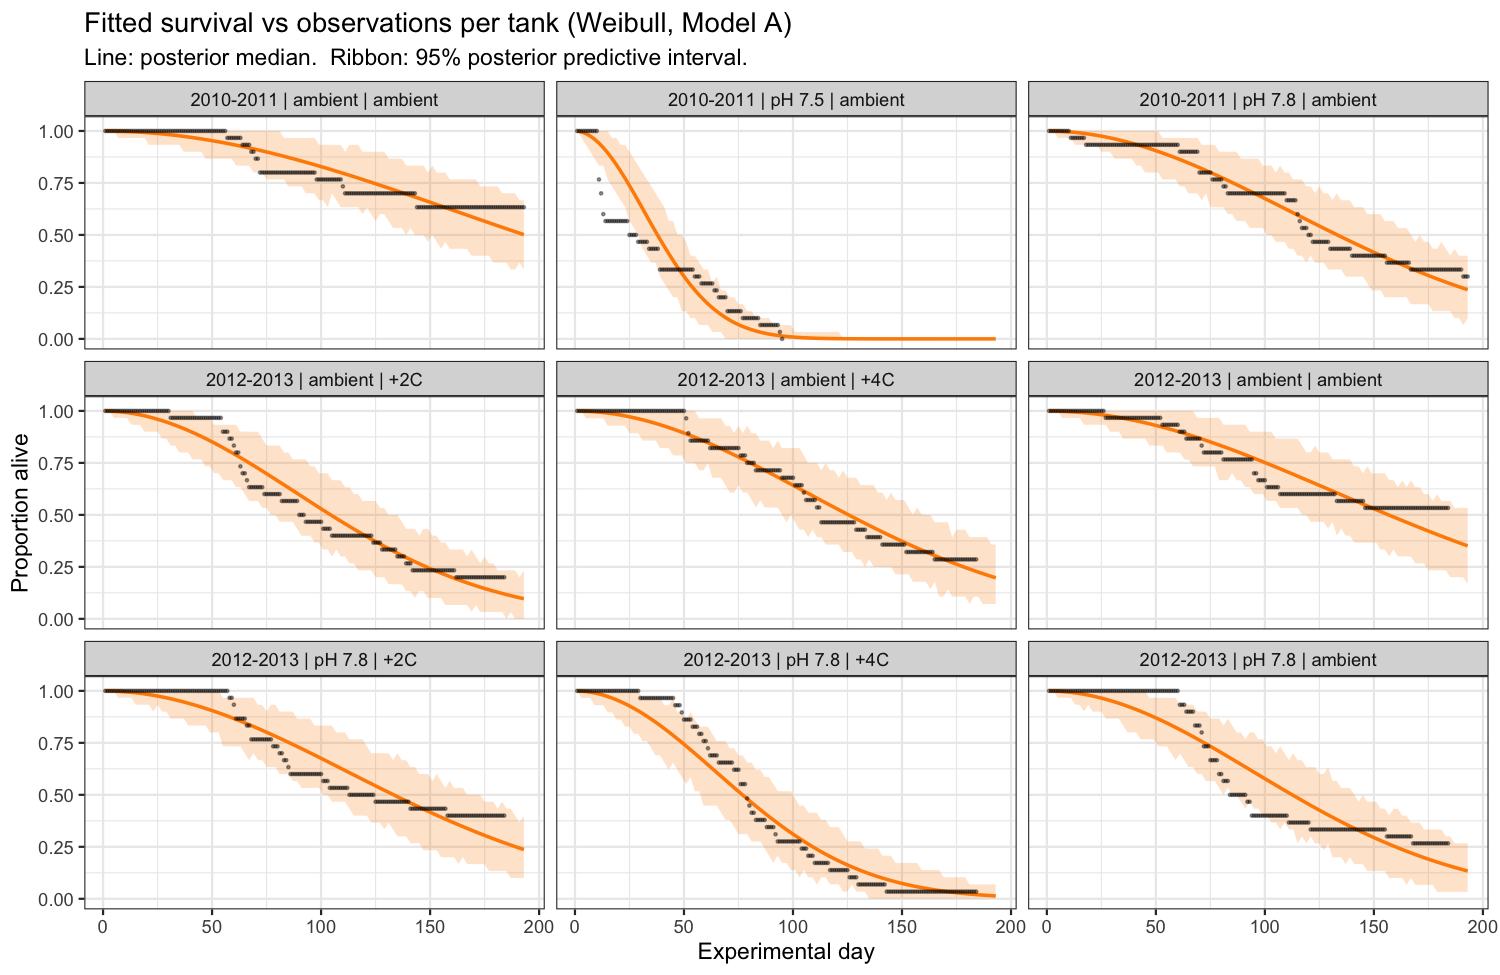
\includegraphics[width=\linewidth]{survival_observed_vs_predicted_weibull.png}
\caption{Survival Model A (Weibull): posterior median (orange line) and 95\% posterior predictive interval (band, incorporating binomial sampling noise from $n = 30$ crabs at the fitted rate), overlaid on observed daily proportions alive (points).}
\label{fig:surv-A}
\end{figure}

\clearpage
\subsection{Survival Model B: all three experiments}
\label{sec:results-b}
Model B extends the experiment factor to three levels. The headline result is a large and credibly negative baseline shift for the 2024--25 experiment relative to 2010 (Table~\ref{tab:surv-B}): $\beta_{\text{exp 2024 vs 2010}} = -2.85$ [$-4.04, -1.62$], corresponding to roughly $9\times$ lower baseline mortality after accounting for pH and temperature. The pH main effect is preserved; the temperature and interaction effects remain centred near zero.

\begin{table}[h]
\centering\small
\begin{tabular}{lrr}
\toprule
Parameter & Median & 95\% CI \\
\midrule
Weibull shape $k$ & 1.98 & 1.94, 2.01 \\
Intercept (log $r$ at pH 8.0, 10$^\circ$C, 2010) & $-10.12$ & $-11.47, -8.83$ \\
Experiment 2012 vs 2010 & $-0.09$ & $-1.47, 1.25$ \\
Experiment 2024 vs 2010 & $-2.85$ & $-4.04, -1.62$ \\
pH (per unit; centred at 8.0) & $-3.00$ & $-6.24, 0.39$ \\
Temperature (per $^\circ$C; centred at 10$^\circ$C) & $-0.11$ & $-0.69, 0.48$ \\
pH $\times$ Temperature interaction & $-0.69$ & $-2.92, 1.52$ \\
Tank-level SD & 0.89 & 0.59, 1.38 \\
\bottomrule
\end{tabular}
\caption{Survival Model B (Weibull) fixed-effect posteriors.}
\label{tab:surv-B}
\end{table}

\begin{figure}[h]
\centering
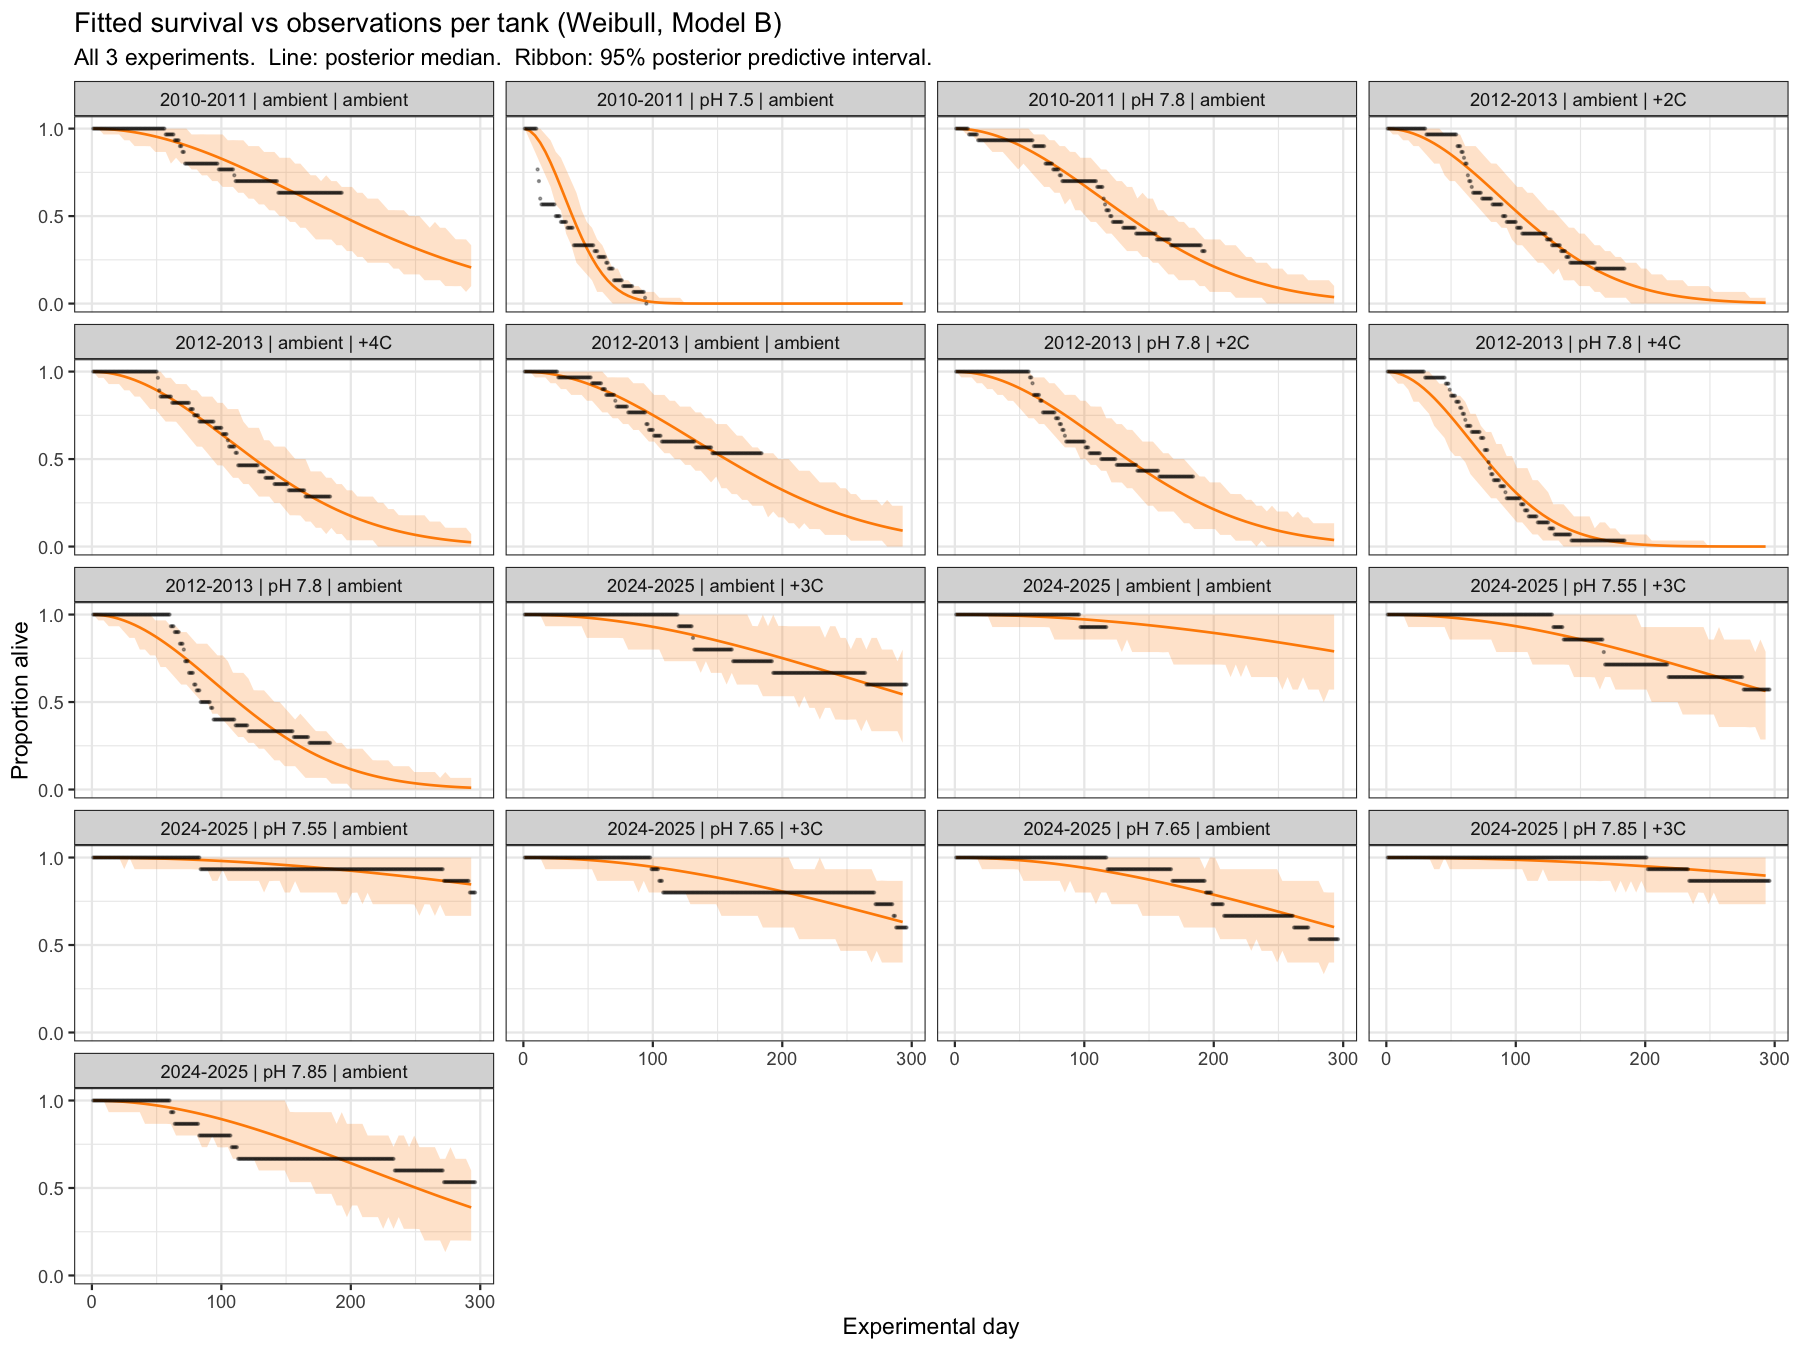
\includegraphics[width=\linewidth]{survival_observed_vs_predicted_weibull_all3.png}
\caption{Survival Model B (Weibull): observed and fitted survival per tank, all three experiments. The 2024 panels (rows 3--5) sit visibly higher than the 2010 and 2012 panels at comparable days. The ambient/ambient 2024 panel ends at day~117 by design (flow-failure censoring).}
\label{fig:surv-B}
\end{figure}

\clearpage
\subsection{Does initial mass mediate the experiment effects on survival?}
\label{sec:results-mass-surv}
The Weibull Models A and B were re-fit with the tank-level centred log mean initial mass added to the linear predictor. LOO shows essentially no improvement from the covariate ($\Delta$ELPD $= -0.2$ in Model A; $-0.4$ in Model B). More importantly, the experiment-level dummy coefficients are essentially unchanged when initial mass is included: the 2024 vs 2010 contrast in Model B moves from $-2.85$ to $-2.83$. Initial size therefore cannot mediate the 2024 baseline shift, consistent with the biological pattern (2010 and 2024 crabs were the same starting size but 2024 had dramatically lower mortality).

\subsection{Growth Model A: published experiments only}
Both growth Models A and B converged cleanly (max $\hat R \le 1.005$; minimum bulk ESS $\ge 2{,}094$). Table~\ref{tab:growth-A} reports the fixed-effect posteriors. The baseline daily growth rate on the log-mass scale is $5.46 \times 10^{-3}$ [4.65, 6.28] $\times 10^{-3}$ --- roughly 0.55\% mass increase per day. The 2012 experiment grows credibly more slowly than 2010 by $1.67 \times 10^{-3}$ log-mass per day. The pH and temperature growth-rate effects are positively signed but their 95\% credible intervals just touch zero.

\begin{table}[h]
\centering\small
\begin{tabular}{lrr}
\toprule
Parameter & Median & 95\% CI \\
\midrule
Baseline growth rate (log-mass per day) & $5.46 \times 10^{-3}$ & $4.65, 6.28 \times 10^{-3}$ \\
$\times$ experiment 2012 vs 2010 & $-1.67 \times 10^{-3}$ & $-2.61, -0.73 \times 10^{-3}$ \\
$\times$ pH (per unit; centred at 8.0) & $2.93 \times 10^{-3}$ & $-0.81, 6.77 \times 10^{-3}$ \\
$\times$ temperature (per $^\circ$C; centred at 10$^\circ$C) & $-1.94 \times 10^{-4}$ & $-6.60 \times 10^{-4}, 2.57 \times 10^{-4}$ \\
$\times$ pH $\times$ T interaction & $-9.54 \times 10^{-4}$ & $-3.99 \times 10^{-3}, 2.06 \times 10^{-3}$ \\
Crab-level SD (log mass) & 0.229 & 0.201, 0.260 \\
Tank-level SD (log mass) & 0.049 & 0.002, 0.210 \\
\bottomrule
\end{tabular}
\caption{Growth Model A fixed-effect posteriors. Growth-rate terms (day-interactions): each value represents an additive contribution to the log-mass slope per day.}
\label{tab:growth-A}
\end{table}

\begin{figure}[h]
\centering
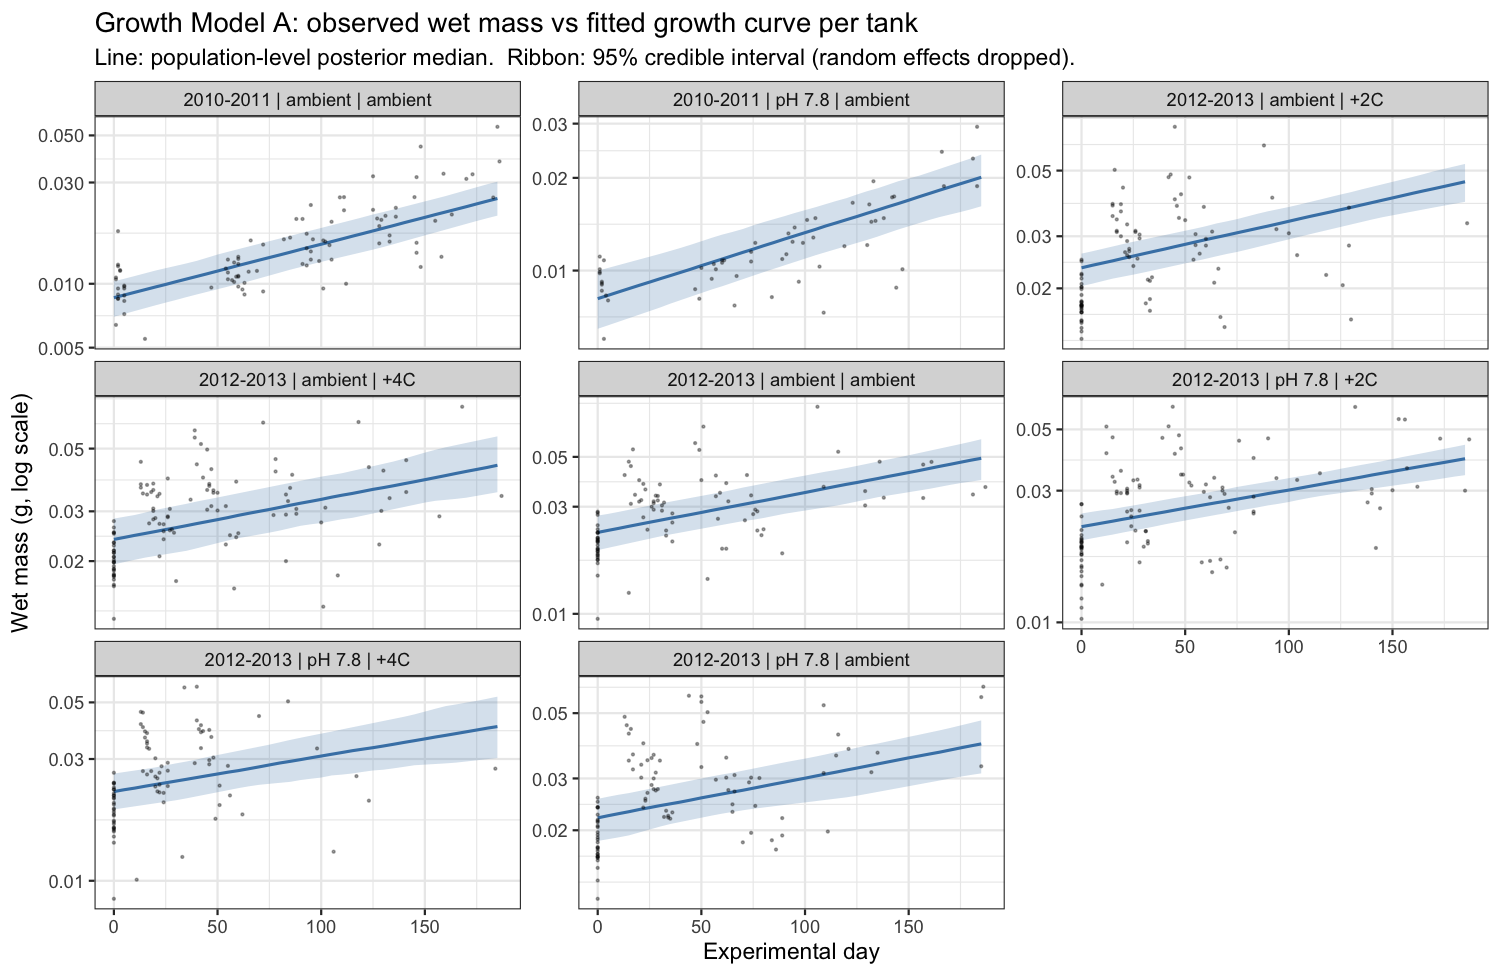
\includegraphics[width=\linewidth]{growth_observed_vs_predicted.png}
\caption{Growth Model A: observed wet masses (points, log scale) and the population-level posterior median growth curve (line) with 95\% credible interval (band) per tank.}
\label{fig:growth-A}
\end{figure}

\clearpage
\subsection{Growth Model B: all three experiments}
\label{sec:results-growth-b}
Adding the 2024--25 data sharpens the inference substantially (Table~\ref{tab:growth-B}). Both the pH and the temperature growth-rate effects are now credibly positive: higher pH and warmer temperatures both increase growth rate. The 2012 experiment growth-rate deficit relative to 2010 is reinforced ($-2.24 \times 10^{-3}$ log-mass per day; 95\% CI $[-3.29, -1.17] \times 10^{-3}$). The 2024 vs 2010 growth-rate contrast is small and uncertain --- 2024 and 2010 crabs grow at similar rates once pH and temperature are accounted for.

\begin{table}[h]
\centering\small
\begin{tabular}{lrr}
\toprule
Parameter & Median & 95\% CI \\
\midrule
Baseline growth rate & $5.94 \times 10^{-3}$ & $5.03, 6.83 \times 10^{-3}$ \\
$\times$ experiment 2012 vs 2010 & $-2.24 \times 10^{-3}$ & $-3.29, -1.17 \times 10^{-3}$ \\
$\times$ experiment 2024 vs 2010 & $0.82 \times 10^{-3}$ & $-0.21, 1.86 \times 10^{-3}$ \\
$\times$ pH & $2.54 \times 10^{-3}$ & $0.17, 4.85 \times 10^{-3}$ \\
$\times$ temperature & $4.46 \times 10^{-4}$ & $0.77, 8.31 \times 10^{-4}$ \\
$\times$ pH $\times$ T interaction & $6.37 \times 10^{-4}$ & $-6.66 \times 10^{-4}, 1.94 \times 10^{-3}$ \\
Crab-level SD (log mass) & 0.262 & 0.237, 0.290 \\
Tank-level SD (log mass) & 0.118 & 0.058, 0.227 \\
\bottomrule
\end{tabular}
\caption{Growth Model B fixed-effect posteriors. \textbf{Both pH and temperature day-interaction terms credibly exclude zero}: higher pH and warmer temperatures increase log-mass growth rate.}
\label{tab:growth-B}
\end{table}

\begin{figure}[h]
\centering
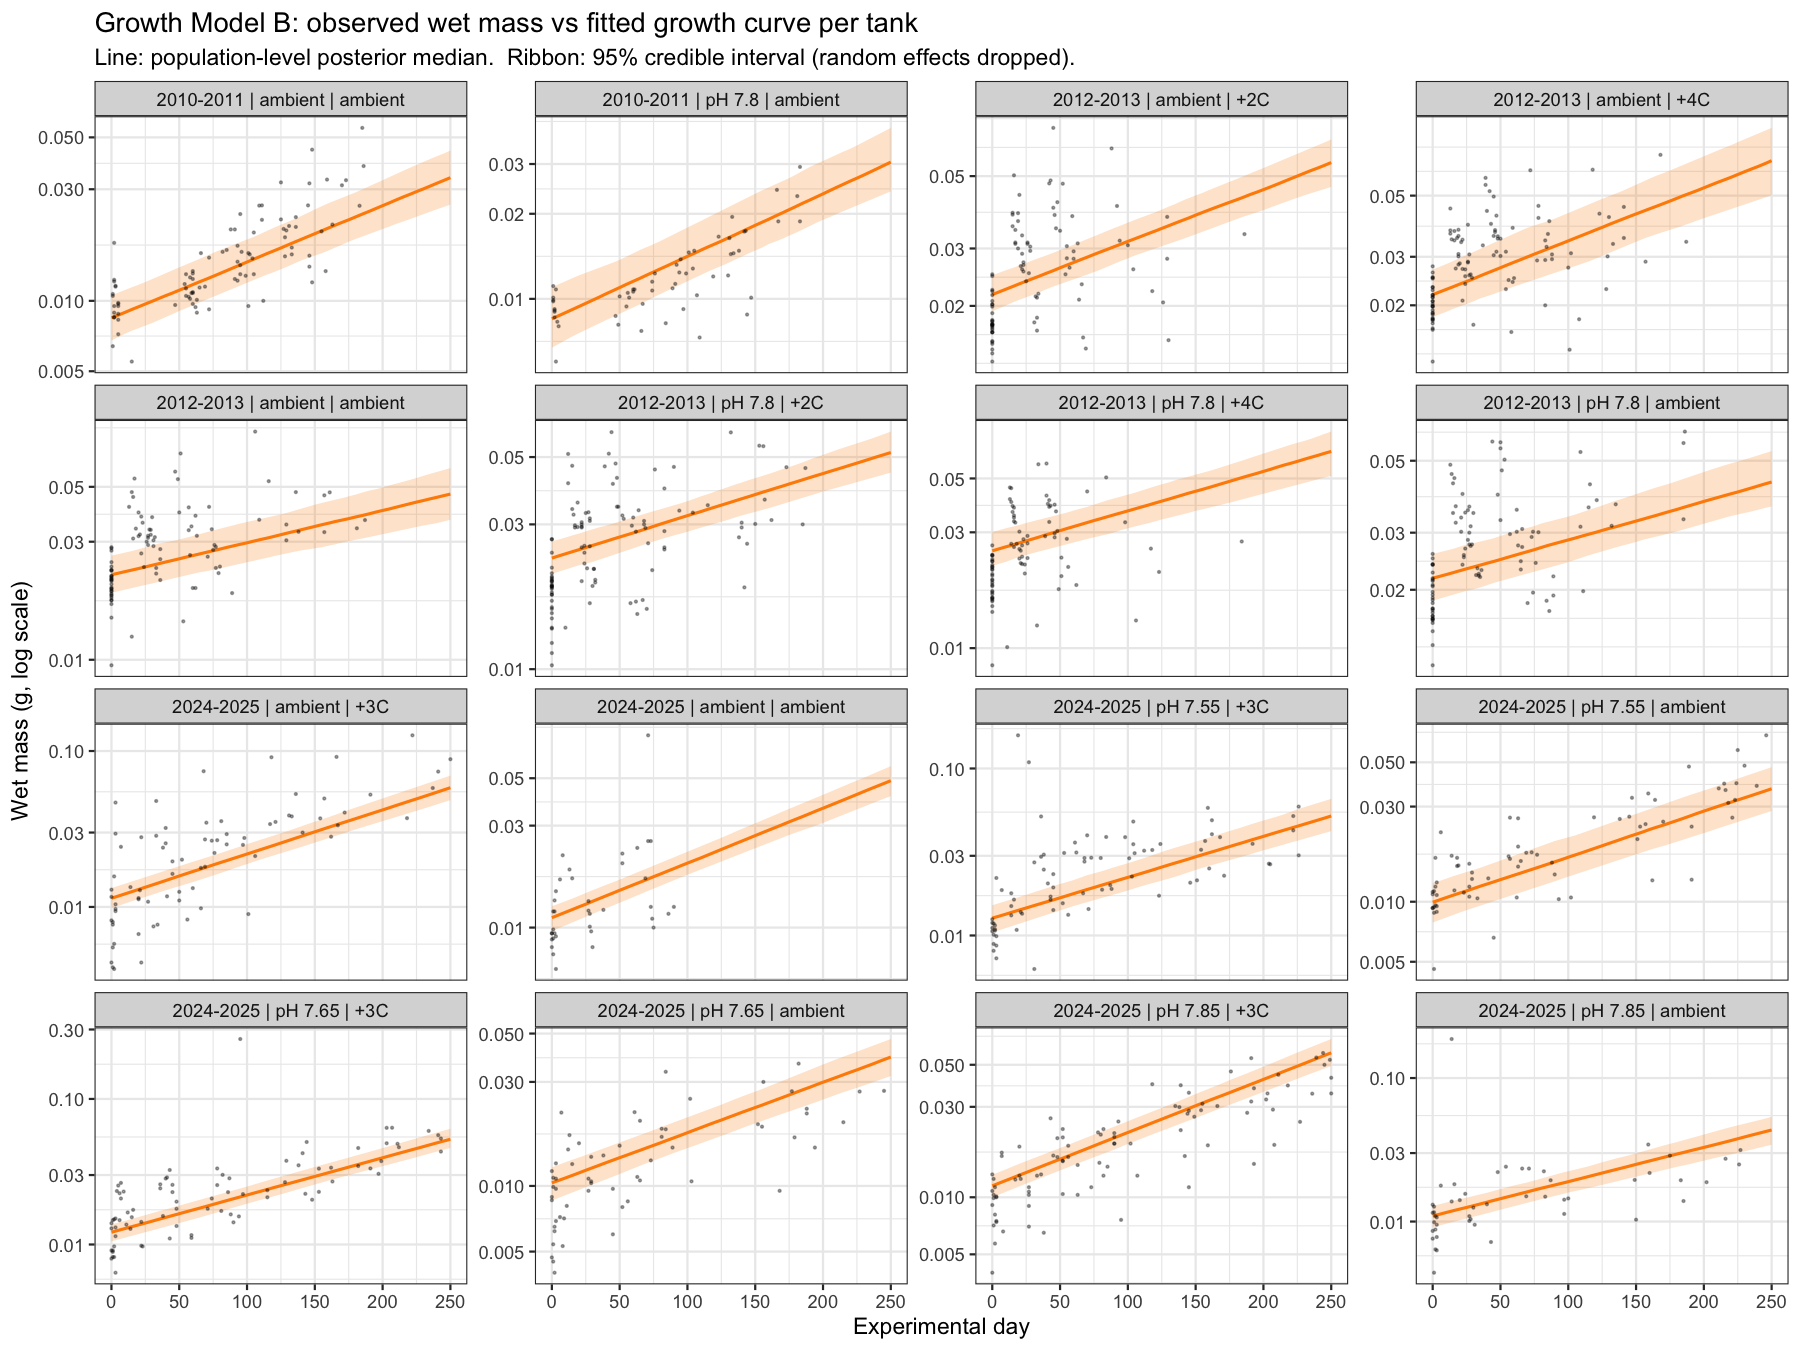
\includegraphics[width=\linewidth]{growth_observed_vs_predicted_all3.png}
\caption{Growth Model B: observed wet masses and fitted population-level growth curves per tank, all three experiments. 2012 tanks (row 2) have visibly flatter slopes than 2010 (row 1, panels 1--2) and 2024 (rows 3--5).}
\label{fig:growth-B}
\end{figure}

\begin{figure}[h]
\centering
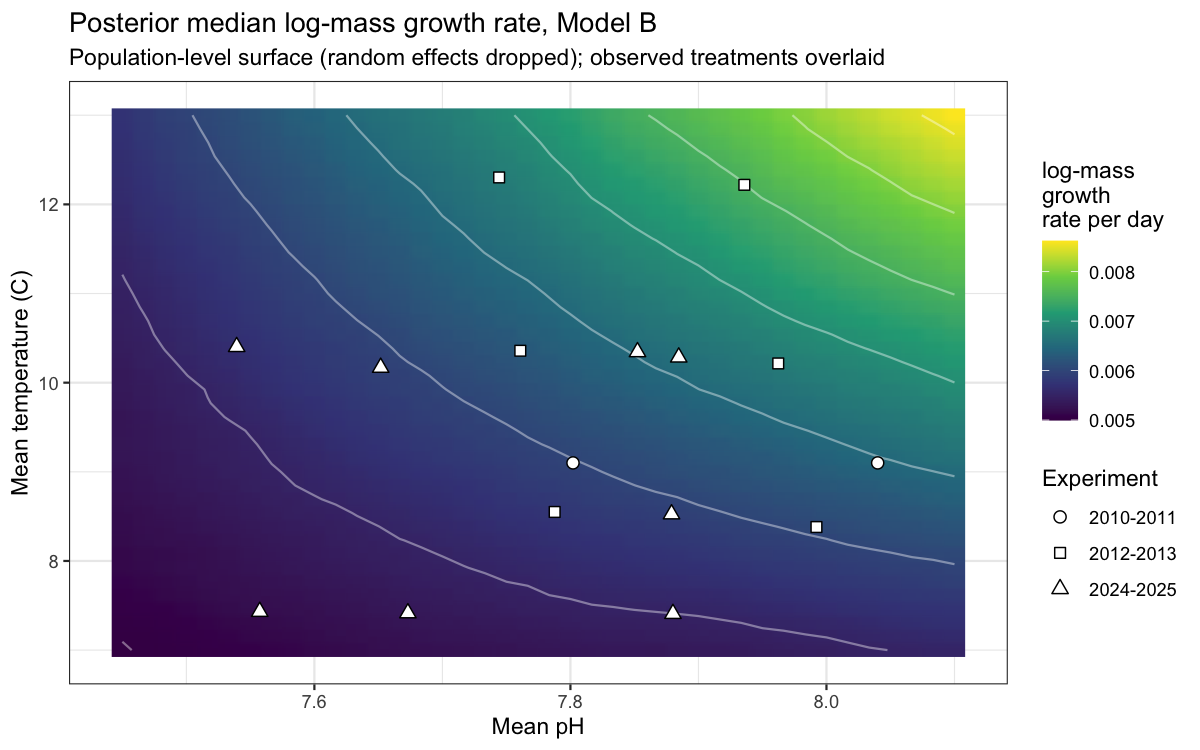
\includegraphics[width=0.85\linewidth]{growth_rate_surface_all3.png}
\caption{Growth Model B posterior median log-mass growth rate (per day) over the realised pH$\times$temperature space. Contours run lower-left (low pH, cold) to upper-right (high pH, warm); the surface is monotonically increasing in both axes. Observed treatments overlaid by experiment.}
\label{fig:growth-surface}
\end{figure}

\clearpage
\subsection{Does starting weight explain the growth differences among years?}
\label{sec:results-mass-growth}
The 2012 cohort grew credibly slower than 2010 and 2024 (Tables~\ref{tab:growth-A}--\ref{tab:growth-B}). A natural biological hypothesis is allometric: 2012 crabs started about twice as heavy as 2010 and 2024 crabs, and proportional (log-mass) growth typically slows with size in crustaceans. To test this, both models were re-fit with the centred log tank-mean initial mass added as both an intercept term and a growth-rate term:
\begin{equation}
\log(\text{WM}_{c,t}) = \cdots + \delta_M \log(M_i) \cdot \text{day}_{c,t} + \cdots,
\end{equation}
where $M_i$ is the centred log tank-mean initial wet mass.

LOO comparison (Table~\ref{tab:loo-growth-mass}) shows essentially no improvement in Model A and only a modest improvement in Model B (1.5 SE). The bigger result is in the coefficient table (Table~\ref{tab:growth-mass-compare}): \textbf{the experiment 2012 vs 2010 day-interaction does not shrink when mass is added} --- in Model B it grows in absolute value from $-2.24 \times 10^{-3}$ to $-5.99 \times 10^{-3}$. The mass day-interaction itself is credibly positive in Model B ($+5.62 \times 10^{-3}$ log-mass per day per unit log tank-mean mass, 95\% CI $[+2.31, +8.89] \times 10^{-3}$).

\begin{table}[h]
\centering\small
\begin{tabular}{llrr}
\toprule
Comparison & Model & $\Delta$ ELPD & SE \\
\midrule
Growth Model A & growth (no mass) & 0 & 0 \\
                & growth $+$ mass & $-1.5$ & 0.7 \\
\midrule
Growth Model B & growth $+$ mass & 0 & 0 \\
                & growth (no mass) & $-5.3$ & 3.6 \\
\bottomrule
\end{tabular}
\caption{LOO comparison of growth models with and without the tank-level initial-mass day-interaction.}
\label{tab:loo-growth-mass}
\end{table}

\begin{table}[h]
\centering\small
\begin{tabular}{lrr}
\toprule
Day-interaction term & No mass covariate & With mass covariate \\
\midrule
$\times$ experiment 2012 vs 2010 ($\times 10^{-3}$) & $-2.24$ [$-3.29$, $-1.17$] & $-5.99$ [$-8.46$, $-3.54$] \\
$\times$ experiment 2024 vs 2010 ($\times 10^{-3}$) & $0.82$ [$-0.21$, $1.86$] & $0.80$ [$-0.24$, $1.82$] \\
$\times$ pH ($\times 10^{-3}$) & $2.54$ [$0.17$, $4.85$] & $2.99$ [$0.72$, $5.26$] \\
$\times$ temperature ($\times 10^{-4}$) & $4.46$ [$0.77$, $8.31$] & $3.53$ [$-0.32$, $7.52$] \\
$\times$ pH $\times$ T interaction ($\times 10^{-3}$) & $0.64$ [$-0.67$, $1.94$] & $0.66$ [$-0.68$, $1.95$] \\
$\times$ log tank-mean initial mass ($\times 10^{-3}$) & --- & $+5.62$ [$+2.31$, $+8.89$] \\
\bottomrule
\end{tabular}
\caption{Posterior median [95\% CI] for the Model B day-interaction (growth-rate) terms with and without the initial-mass covariate. The 2012-vs-2010 effect grows in absolute value rather than shrinking.}
\label{tab:growth-mass-compare}
\end{table}

Read together, these results indicate that \textbf{starting weight does not explain the among-year growth differences}. The pattern is a classic statistical suppression: the raw between-experiment correlation between mass and growth is negative (2012 had heavy, slow-growing crabs; 2010 and 2024 had lighter, faster-growing crabs), but that is a cohort confound, not allometry. When mass is included as a covariate, the residual within-design mass-vs-growth-rate relationship is positive, and the pure 2012-cohort effect --- everything that distinguishes the 2012 experiment from 2010 \textit{besides} starting size --- becomes larger, not smaller. If 2012 crabs were slow growers because they were big, the experiment dummy should have shrunk; instead it nearly tripled in magnitude.

The proper way to test allometric scaling is at the \textbf{within-crab} level, in a model where each crab's instantaneous growth rate depends on its current mass --- not at the tank-mean aggregate. With seventeen tank-level mass values and 335 crabs, a von Bertalanffy or Weibull-style growth function fitted to individual trajectories would have far more leverage. That extension is recommended in §\ref{sec:nextsteps}(a).

\clearpage
\subsection{Threshold pH effects (smooth analysis)}
\label{sec:threshold}
The 2024--25 experiment was specifically designed with four pH levels (7.55, 7.65, 7.85, ambient at ${\approx}\,7.88$) crossed with two temperatures, giving the resolution to detect a threshold or other nonlinear pH effect. To test for one, the linear pH terms (and the pH$\times$T interaction) in both survival and growth models were replaced by a Bayesian thin-plate spline over mean pH (§\ref{sec:smooth_model}). LOO comparison of smooth vs linear is reported in Table~\ref{tab:loo-smooth}.

\begin{table}[h]
\centering\small
\begin{tabular}{llrr}
\toprule
Response & Design & $\Delta$ ELPD (smooth $-$ linear) & SE \\
\midrule
Survival & Model A & $-0.2$ & 0.1 \\
Survival & Model B & 0.0    & 0.1 \\
Growth   & Model A & $+2.6$ & 2.1 \\
Growth   & Model B & $+2.0$ & 2.2 \\
\bottomrule
\end{tabular}
\caption{LOO comparison of smooth-pH vs linear-pH formulations. None of the differences exceeds 1.5~SE.}
\label{tab:loo-smooth}
\end{table}

\textbf{None of the LOO differences are decisive}, and the posterior smooth shapes (Figures~\ref{fig:smooth-surv} and \ref{fig:smooth-growth}) show monotonic, near-linear behaviour rather than threshold inflections. For survival the smooth declines roughly linearly across the realised pH range in both designs (more sharply in Model A because the 2010 pH~7.5 cohort anchors the low-pH end at high mortality). For growth the smooth is essentially flat across pH 7.5--7.9 with a slight upturn near pH~8.0, but the upturn is in the region where only the 2010 ambient tank contributes data and the credible interval is wide.

\begin{figure}[h]
\centering
\begin{minipage}{0.49\linewidth}
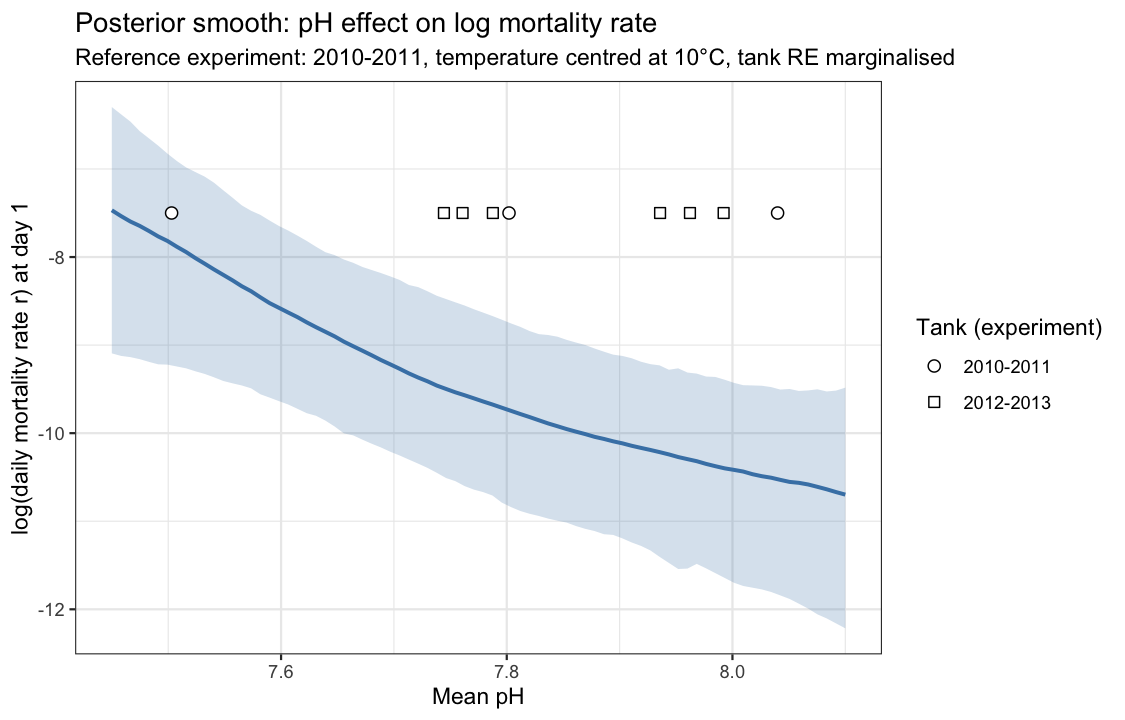
\includegraphics[width=\linewidth]{survival_smooth_pH.png}
\end{minipage}\hfill
\begin{minipage}{0.49\linewidth}
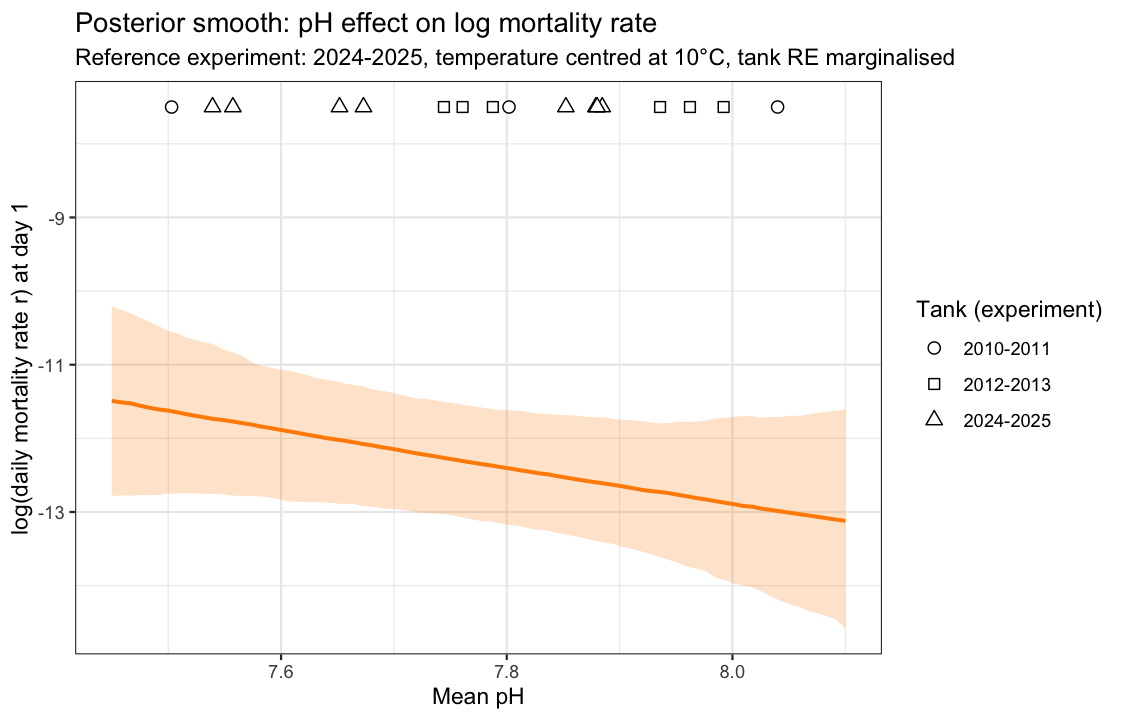
\includegraphics[width=\linewidth]{survival_smooth_pH_all3.png}
\end{minipage}
\caption{Posterior smooth of log mortality rate against mean pH for the published-only Model A (left) and the all-three-experiment Model B (right). Random effects marginalised. Both smooths are monotonic; neither shows a threshold inflection.}
\label{fig:smooth-surv}
\end{figure}

\begin{figure}[h]
\centering
\begin{minipage}{0.49\linewidth}
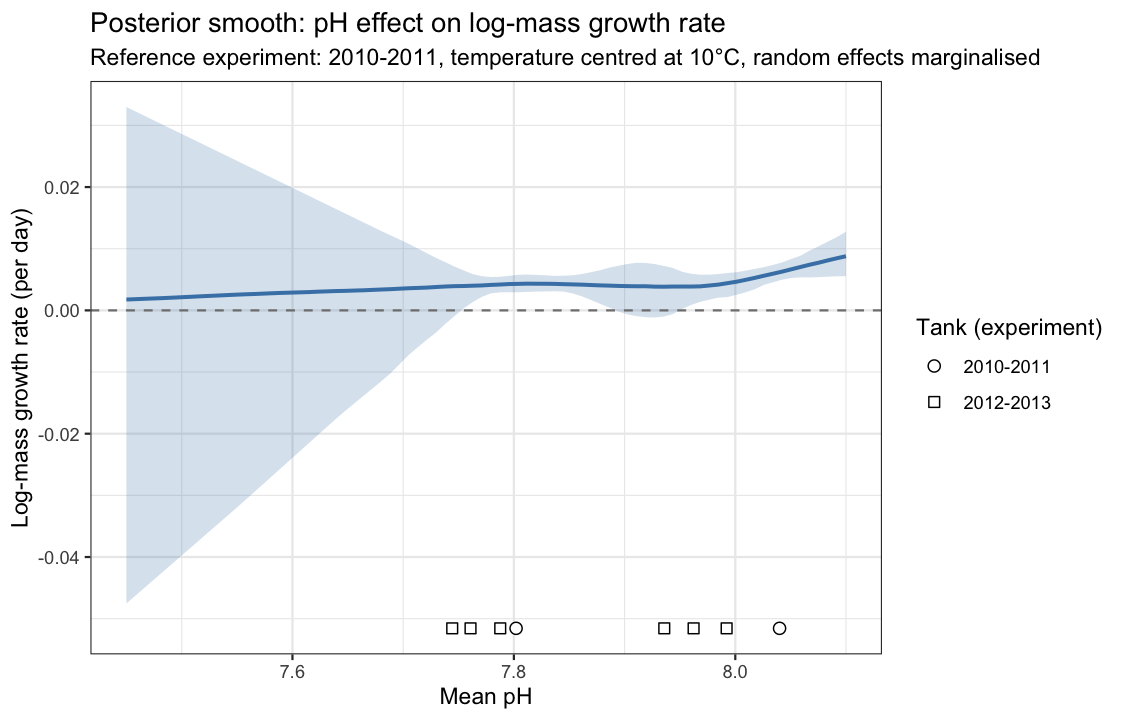
\includegraphics[width=\linewidth]{growth_smooth_pH.png}
\end{minipage}\hfill
\begin{minipage}{0.49\linewidth}
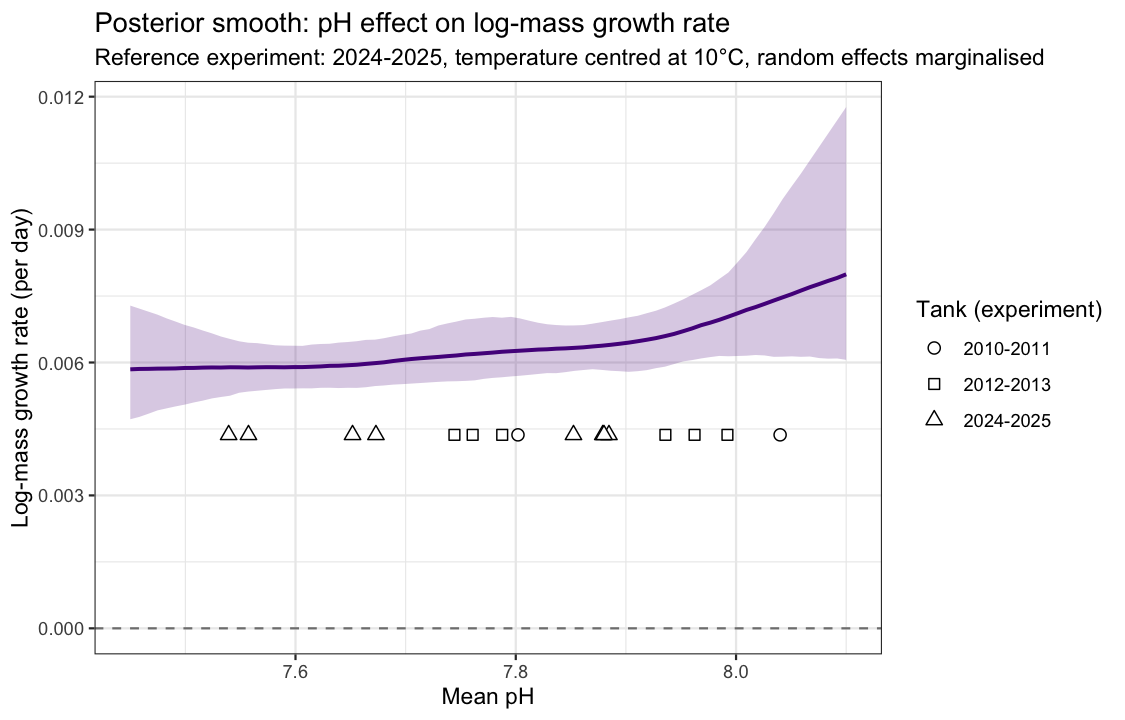
\includegraphics[width=\linewidth]{growth_smooth_pH_all3.png}
\end{minipage}
\caption{Posterior smooth of log-mass growth rate against mean pH for Model A (left) and Model B (right). Random effects marginalised. The growth-rate surface is essentially flat across the well-sampled pH range; the upturn near ambient pH in Model B is poorly identified.}
\label{fig:smooth-growth}
\end{figure}

The data therefore \textbf{do not support a threshold pH response} for either survival or growth at the resolution of the realised treatments. The pH effect is approximately monotonic: lower pH increases mortality, and at the pH values realised here it has a weak, roughly linear effect on growth rate. The conclusion may change with a wider pH range; the realised low extreme in 2024 (${\approx}\,7.54$) is well above the 2010 low (${\approx}\,7.50$), so the joint dataset still lacks resolution below pH~7.5 where the 2010 cliff occurred.

% ============================================================
\clearpage
\section{Discussion}
% ============================================================

\subsection{The hazard is not constant in time}
The single largest methodological result is that the constant-hazard parameterisation used in both source papers is materially wrong for these data. The Weibull formulation improves out-of-sample predictive performance by more than 1{,}400 ELPD units in Model A and more than 1{,}700 in Model B. The shape parameter $k \approx 2$ implies that daily mortality risk increases roughly linearly with time-since-start: the population is not in stationary equilibrium. Rate-based summaries that assume stationarity (including those in the source papers) systematically understate late-experiment mortality and overstate early-experiment mortality.

\subsection{Survival: Model A vs Model B}
\textbf{The pH signal on survival is robust.} $\beta_{\text{pH}} \approx -3$ in Model B and $\approx -4$ in Model A, both with credible intervals well below zero. Higher pH lowers daily mortality.

\textbf{The temperature signal on survival remains weak.} No credible main effect or interaction in either design.

\textbf{The 2024 baseline is conspicuously low and is not explained by initial mass.} 2024 tanks all have lower posterior mortality rates than the 2010 and 2012 controls. Including initial wet mass as a tank-level covariate does not change the experiment effect or improve predictive performance.

\subsection{Growth: Model A vs Model B}
The growth analysis recovers a story complementary to the survival results. \textbf{2012 crabs grow credibly slower than 2010 and 2024} (Model B: $\delta_{2012} = -2.24 \times 10^{-3}$, 95\% CI $[-3.29, -1.17] \times 10^{-3}$). 2010 and 2024 grow at indistinguishable rates after adjustment.

\textbf{The pH and temperature effects on growth are credibly positive in Model B}, while Model A could not resolve them. Higher pH and warmer temperatures both increase growth rate. The pH effect on growth is in the same direction as the pH effect on survival: low-pH water both increases mortality and slows growth.

A natural first hypothesis for the 2012 growth-rate deficit was allometric, but the mass-mediation test in §\ref{sec:results-mass-growth} rejects this at the tank-aggregate level: including tank-mean initial mass \textit{increases} rather than absorbs the 2012-vs-2010 contrast. The 2012 deficit is therefore a cohort/experiment property, not a size property --- consistent with the parallel result for survival.

\subsection{Threshold effects}
The 2024 design supplied the pH resolution to look for threshold responses. Across both survival and growth, the data are consistent with monotonic, approximately linear effects of pH on the log mortality-rate and log-mass growth-rate scales. Neither smooth shows an inflection in the realised pH range (7.5--8.0). This is a useful null result, but it does not rule out threshold behaviour below pH 7.5, which lies outside the joint coverage of the three experiments.

\subsection{The survival/growth picture in 2024}
2024 crabs had the lowest mortality and (jointly with 2010) the highest growth rate of any of the seventeen tanks. Initial wet mass does not explain this: 2024 and 2010 started at similar sizes but 2024 mortality was an order of magnitude lower. The most plausible explanations are biological/husbandry rather than physiological: the 2024 cohort was laboratory-reared from a single ovigerous female (2010 and 2012 used field-collected juveniles); the diet recipe included astaxanthin supplementation that the earlier experiments lacked; and water source and seasonal conditions have shifted measurably over the decade. The current models absorb these unknowns into the experiment-level intercept; pH and temperature slopes are conditional on that baseline.

\subsection{Next steps}
\label{sec:nextsteps}
\noindent\textbf{(a) Allometric growth.} The log-linear growth model is a first approximation. Crustacean growth typically decelerates with size, which should be added as an allometric exponent --- either $\log(\text{WM}) \sim \lambda \log(\text{day})$ or a von Bertalanffy formulation. The current tank-mean mass-mediation test (§\ref{sec:results-mass-growth}) is the coarse version; a within-crab implementation would have substantially more leverage to detect size-dependence.

\noindent\textbf{(b) Time-varying covariates.} The Weibull formulation captures increasing hazard but assumes pH and temperature effects do not themselves vary with time. A future extension could let $\beta_{\text{pH}}$ interact with $\log t$, testing whether low-pH effects compound over time.

\noindent\textbf{(c) Investigation of the 2024 baseline shift.} If covariates describing cohort source, diet composition, salinity, or starting weight at deeper resolution are available from laboratory notebooks, they could be added in place of the experiment dummy. The work in §\ref{sec:results-mass-surv} shows that tank-level initial mass is not such a covariate.

% ============================================================
\section{Reproducibility}
% ============================================================

All steps are reproducible from the repository \texttt{juvenile-RKC-OA-experiments}:
\begin{itemize}
\item \texttt{scripts/data\_wrangling.R} --- ingest the CSVs, document corrections, and write harmonised tables to \texttt{data/combined/}.
\item \texttt{scripts/check\_against\_papers.R} --- refit the published models on the cleaned data and compare to Long et al.\ 2013 and Swiney et al.\ 2017.
\item \texttt{scripts/survival.R} --- fit the constant-hazard, Weibull, Weibull+mass, and smooth-pH versions of Models A and B; perform LOO comparisons; save fits to \texttt{output/models/}; write figures to \texttt{output/figures/}.
\item \texttt{scripts/growth.R} --- fit the log-linear growth, growth+mass, and smooth-pH growth models for Models A and B.
\item \texttt{documents/session\_transcript.md} --- complete conversational record of the analytical work.
\end{itemize}

\end{document}
